\chapter{Podstawy}
\thispagestyle{chapterBeginStyle}

Aby w pełni móc zrozumieć przekrój problemów jaki poruszymy, niezbędne jest uprzednie zapoznanie się z podstawami, na których są one oparte. Jako, że będziemy rozważali problemy odpornej optymalizacji na przykładzie minimalnych drzew rozpinających, w tym rozdziale zajmiemy się przedstawieniem podstawowych definicji dotyczących zagadnień bezpośrednio nimi związanych. Przytoczymy definicje samego \textbf{minimalnego drzewa rozpinającego} (ang. \textit{minimum spanning tree}), \textbf{grafów}, terminów im pochodnych oraz sposobów ich reprezentacji. Na samym końcu dokonamy przeglądu algorytmów do rozwiązywania problemu minimalnego drzewa rozpinającego (dalej będziemy często wykorzystywać skrót od ich angielskiej nazwy --- \textbf{MST}) oraz przyjrzymy się właściwościom tych specyficznych struktur grafowych, na podstawie których wspomniane algorytmy funkcjonują i zwracają poprawne rozwiązania.

\section{Grafy a drzewa rozpinające}

Chcąc mówić o problemie \textbf{minimalnego drzewa rozpinającego} musimy najpierw przypomnieć sobie definicje podstawowych zagadnień związanych z grafami. \textbf{Grafem} $G = \left( V, E \right)$ będziemy zatem nazywać zbiór punktów $v_{i} \in V$ opcjonalnie ze sobą połączonych krawędziami $e_{ij} \in E$, gdzie przyjmiemy następującą definicję krawędzi: $e_{ij} \equiv v_{i} \overset{1}{\leadsto} v_{j}$, która wyraża fakt istnienia łuku (krawędzi) pomiędzy wierzchołkami (punktami) grafu $v_{i}$ oraz $v_{j}$, które są nim bezpośrednio połączone\footnote{Wyrażeniem $v_{i} \overset{k}{\leadsto} v_{j}$ często też będziemy chcieli zaznaczać fakt istnienia \textbf{ścieżki} pomiędzy wierzchołkami $v_{i}$ a $v_{j}$, gdzie $k$ oznaczać będzie dokładną liczbę krawędzi, która znajduje się na takiej ścieżce między wymienionymi wierzchołkami (jeśli $k = \ast$, wtedy ich liczba może być dowolna, dla $k = 1$ będziemy tę liczbę pomijać). \textbf{Ścieżką} pomiędzy wierzchołkami $v_{i}$ oraz $v_{j}$ będziemy zaś nazywać następujący ciąg krawędzi: $\left\{ v_{i} \overset{1}{\leadsto} v_{a_{1}}, v_{a_{1}} \overset{1}{\leadsto} v_{a_{2}}, \dots, v_{a_{b}} \overset{1}{\leadsto} v_{a_{b+1}}, v_{a_{b+1}} \overset{1}{\leadsto} v_{j}  \right\}$.}. Same zaś wierzchołki będziemy numerować za pomocą indeksów $i \in \left\{ 1, \dots, \left| V \right| \right\}$, gdzie $\left| V \right| = n$ i wyraża \textbf{moc} (liczbę elementów) zbioru wierzchołków grafu. Analogicznie będziemy przyjmować, że $\left| E \right| = m$. 

Przy omawianiu problemu \textbf{minimalnego drzewa rozpinającego} będziemy rozważać tylko specyficzną rodzinę grafów: grafów nieskierowanych (ang. \textit{undirected graphs}), które charakteryzują się tym, że fakt istnienia krawędzi $e_{ij}$ pomiędzy wierzchołkami grafu $v_{i}$ oraz $v_{j}$ nie przesądza o \textbf{kierunku} danego łuku --- w przypadku grafu nieskierowanego nasza definicja łuku tak naprawdę powinna wyglądać następująco: $e_{ij} \equiv v_{i} \overset{1}{\leadsto} v_{j} \wedge v_{j} \overset{1}{\leadsto} v_{i}$ (zatem w grafie nieskierowanym $e_{ij} \equiv e_{ji}$, zaś stosowana w zapisie kolejność indeksów jest tylko umowna). Będziemy wymiennie, w zależności od sytuacji, stosować aż cztery rodzaje oznaczeń krawędzi $e$:
\begin{itemize}
	\item $e_{ij}$, gdy będziemy chcieli podkreślić fakt wystąpienia krawędzi pomiędzy wierzchołkami grafu o indeksach $i$ oraz $j$,
	\item $\left( i, j \right)$, gdy będziemy chcieli położyć szczególny nacisk na połączone ze sobą wierzchołki grafu,
	\item $e_{i}$, gdzie w tym przypadku $i \in \left\{ 1, \dots, \left| E \right| \right\}$ oznacza indeks krawędzi w grafie, oraz $v_{i} \overset{1}{\leadsto} v_{j}$, gdy będziemy chcieli albo podkreślić rozpatrywany przez nas ,,kierunek'' krawędzi nieskierowanej.
\end{itemize}
Dodatkowo każda krawędź będzie posiadała dodatkowy atrybut, zwany przez nas dalej \textbf{kosztem} (lub \textbf{wagą}) krawędzi. Jako że bierzemy pod uwagę tylko grafy nieskierowane, koszty krawędzi $e_{ij}$ oraz $e_{ji}$ z definicji są takie same. Wagi krawędzi $e_{ij}$ będziemy oznaczać jako $c_{e_{ij}}$ (ang. \textit{cost}) lub jako $c_{e}$ (w przypadku, gdy nie będą nas interesowały wierzchołki które dana krawędź łączy), lub jako $c_{k}$ (gdy będziemy chcieli odwołać się do kosztu krawędzi $e$ o indeksie $k$). Pełną zatem definicją krawędzi w grafie nieskierowanym przedstawia równość:

\begin{equation}
e_{ij} \equiv v_{i} \overset{1, c_{ij}}{\leadsto} v_{j} \; \wedge ; v_{j} \overset{1, c_{ij}}{\leadsto} v_{i}
\end{equation}

Różnicę między grafami skierowanymi a nieskierowanymi przedstawiają rysunki \ref{fig:dagudacExample:a} oraz \ref{fig:dagudacExample:b} --- w drugim przypadku widzimy, że wiele ścieżek, możliwych do skonstruowania dla grafu nieskierowanego, jest nieosiągalnych w przypadku nadania krawędziom kierunku. Dodatkowo ważnym założeniem które przyjmiemy, będzie brak występowania w grafie wielu krawędzi o wspólnym wierzchołku początkowym oraz końcowym, czyli: $\left( e_{i} \equiv v_{s_{i}} \leadsto v_{t_{i}} \neq e_{j} \equiv v_{s_{j}} \leadsto v_{t_{j}} \right) \rightarrow s_{i} \neq s_{j} \vee t_{i} \neq t_{j}$, gdzie $s_{i}, s_{j}$ oznaczają odpowiednio wierzchołki początkowe (źródła --- ang. \textit{sources}) krawędzi $e_{i}$ oraz $e_{j}$, zaś $t_{i}, t_{j}$ --- ich węzły końcowe (cele --- ang. \textit{targets}). Grafy, które nie spełniają tej własności (posiadają więcej niż jedną krawędź prowadzącą bezpośrednio z wierzchołka początkowego $v_{s}$ do węzła końcowego $v_{t}$ nazywamy \textbf{multigrafami} i nie będziemy się nimi zajmować.)

\begin{figure}[!htbp]
	\null\hfill
	\begin{subfigure}[b]{0.32\textwidth}
		\includegraphics[width=\textwidth]{Chapter_I/DAG-UDAG-example/a}
		\caption{}
		\label{fig:dagudacExample:a}
	\end{subfigure}
	\hfill
	\begin{subfigure}[b]{0.32\textwidth}
		\includegraphics[width=\textwidth]{Chapter_I/DAG-UDAG-example/b}
		\caption{}
		\label{fig:dagudacExample:b}
	\end{subfigure}
	\hfill\null
	\caption{
		\textbf{(a)}~Nieskierowany graf $G = \left( V, E \right)$, gdzie $V = \left\{ v_{1}, v_{2}, \dots, v_{8} \right\}$ i $E = \left\{ e_{1}, e_{2}, \dots, e_{11} \right\}$.
		\textbf{(b)}~Skierowana wersja tego samego grafu.
	}
	\label{fig:dagudacExample}
\end{figure}

\subsection{Drzewo rozpinające}

Rozpoczniemy od definicji drzewa, które jest specyficznym rodzajem grafu:

\begin{definition}
	Drzewo jest spójnym grafem nie zawierającym żadnych cykli.
\end{definition}

\textbf{Grafem spójnym} z kolei nazywamy graf, którego wszystkie wierzchołki są ze sobą w dowolny sposób połączone --- do wszystkich z nich jesteśmy w stanie dojść z wykorzystaniem pewnej liczby krawędzi grafu. \textbf{Cyklem} zaś nazywamy taką ścieżkę w grafie, której wierzchołek początkowy jest jednocześnie węzłem na końcu tej ścieżki.

\begin{figure}[!htbp]
	\null\hfill
	\begin{subfigure}[b]{0.32\textwidth}
		\includegraphics[width=\textwidth]{Chapter_I/DEF-example/a}
		\caption{}
		\label{fig:defExample:a}
	\end{subfigure}
	\hfill
	\begin{subfigure}[b]{0.32\textwidth}
		\includegraphics[width=\textwidth]{Chapter_I/DEF-example/b}
		\caption{}
		\label{fig:defExample:b}
	\end{subfigure}
	\hfill
	\begin{subfigure}[b]{0.32\textwidth}
		\includegraphics[width=\textwidth]{Chapter_I/DEF-example/c}
		\caption{}
		\label{fig:defExample:c}
	\end{subfigure}
	\hfill\null
	\caption{
		\textbf{(a)}~Graf nieskierowany $G^{\prime} = \left( V, E \right)$, gdzie $V = \left\{ v_{1}, v_{2}, \dots, v_{8} \right\}$ i $E = \left\{ e_{1}, e_{2}, \dots, e_{11} \right\}$ zawierający $5$ cykli: $\left\{ e_{1}, e_{2}, e_{7}, e_{6}, e_{9}, e_{8}, e_{3} \right\}$, $\left\{ e_{2}, e_{7}, e_{5} \right\}$, $\left\{ e_{2}, e_{7}, e_{6}, e_{4}, e_{1} \right\}$, $\left\{ e_{1}, e_{5}, e_{6} \right\}$, $\left\{ e_{1}, e_{5}, e_{6}, e_{9}, e_{8}, e_{3} \right\}$. Graf jest niespójny --- wierzchołek $v_{7}$ nie jest w żaden sposób połączony z pozostałymi wierzchołkami grafu.
		\textbf{(b)}~Graf skierowany posiadający tylko dwa cykle (zaznaczone czarnym kolorem): $\left\{ e_{2}, e_{7}, e_{5} \right\}$ oraz $\left\{ e_{2}, e_{11}, e_{10}, e_{9}, e_{6}, e_{5} \right\}$.
		\textbf{(c)}~Przykład cięcia w grafie.
	}
	\label{fig:defExample}
\end{figure}

\textbf{Drzewem rozpinającym} dany graf $G = \left( V, E \right)$ będziemy nazywać taki najmniej liczny zbiór krawędzi $T$, który łączy ze sobą wszystkie wierzchołki w grafie. Formanie:

\begin{equation}
	T = \left\{ e \in E : \left| T \right| = \left| V \right| - 1 \wedge \left( \forall v, v^{\prime} \in V : v \neq v^{\prime} \right) \; !\exists v \overset{\ast, T}{\leadsto} v^{\prime} \right\}\text{,}
\end{equation}
gdzie $\left| T \right|$ symbolizuje liczbę krawędzi w zbiorze $T$, $v \overset{\ast, E}{\leadsto} v^{\prime}$ wyraża dowolnej długości ścieżkę składającą się tylko z krawędzi generowanego zbioru $T$. Zbiór ten, jak widać z powyższej definicji, powinien mieć tę własność, że dla dowolnych dwóch różnych wierzchołków należących do grafu, istnieje dokładnie jedna ścieżka pomiędzy tymi wierzchołkami. Aby przekonać się, że liczba krawędzi należących do zbioru $T$ rzeczywiście powinna wynosić $\left| V \right| - 1$, możemy posłużyć się następującą konstrukcją:

\begin{itemize}
	\item poprowadźmy w grafie ścieżkę przechodzącą przez wszystkie wierzchołki dokładnie raz i kończącą się w wierzchołku początkowym (zbudujmy \textbf{cykl Hamiltona}) --- nie trudno zauważyć, że aby połączyć ze sobą wszystkie wierzchołki, potrzebujemy z każdego kolejnego wierzchołka poprowadzić nową krawędź. Otrzymujemy zatem cykl złożony z dokładnie $\left| V \right|$ krawędzi.
	\item Usuńmy teraz dowolną krawędź z cyklu. Ta operacja powoduje oczywiście jego przerwanie, zaś ze sposobu jego konstrukcji wynika, że pozostała ścieżka przechodzi kolejno przez wszystkie węzły w grafie --- tworzy drzewo rozpinające o liczbie krawędzi równej $\left| V \right| - 1$.
\end{itemize}

\section{Problem minimalnego drzewa rozpinającego}

Niech $\mathcal{T}_{G}$ oznacza zbiór wszystkich drzew rozpinających dla grafu $G$. Problem \textbf{minimalnego drzewa rozpinającego} polega na znalezieniu takiego zbioru krawędzi $T^{\ast} \in \mathcal{T}_{G}$, że ich całkowity koszt jest najmniejszy spośród wszystkich pozostałych możliwych rozwiązań. Zanim jednak bezpośrednio przejdziemy do omawiania algorytmów, które służą do odnajdywania konstrukcji o takich właściwościach, przedstawimy warunki jakie musi spełniać drzewo, abyśmy mieli pewność że suma kosztów jego krawędzi rzeczywiście jest najmniejsza.

Pierwszym takim podejściem do zdefiniowania warunków optymalności rozwiązania $T$ jest warunek \textbf{optymalnych cięć}. Zaprezentowany na rysunku \ref{fig:defExample:c} przykład prezentuje cięcie grafu $G$ --- w przypadku cięcia drzew rozpinających takie posunięcie spowoduje jego podział na dwie części, tak jak to pokazano na rysunkach \ref{fig:cut:a}--\ref{fig:cut:c}, gdyż w wyniku zastosowania cięcia przez wybraną krawędź jest ona usuwana z ciętego zbioru. Optymalnym cięciem natomiast będziemy nazywali takie cięcie, w wyniku którego z grafu usuwana jest krawędź o jak najmniejszym (w przypadku problemów minimalizacyjnych) koszcie ze wszystkich znajdujących się na drodze takiego cięcia (np. na rysunku \ref{fig:defExample:c} cięcie przechodzi przez krawędzie $\left\{ e_{1}, e_{6}, e_{10} \right\}$). W przypadku cięcia drzewa rozpinającego $T$ (patrz rysunek \ref{fig:cut}) przez krawędź $e_{6}$, zbiór taki będziemy oznaczać przez $\mathcal{Q} \left( T, e_{6} \right)$ i będą do niego należeć wszystkie krawędzie $e^{\prime} \in E$ łączące ze sobą dwa, powstałe w wyniku cięcia, zbiory wierzchołków, zgodnie z poniższą definicją.

\begin{equation}\label{eq:treecutedgeset}
\mathcal{Q} \left( T, e \right) = \left\{ \left( i, j \right) \; : \; v_{i} \in V_{1} \wedge v_{j} \in V_{2} \right\}
\end{equation}

\begin{theorem}[Kryterium optymalnych cięć (ang. \textit{Cut Optimality Conditions})]\label{def:optmstcut}
	Dla grafu $G = \left( V, E \right)$, drzewo rozpinające $T^{\ast}$ jest minimalnym drzewem rozpinającym dany graf wtedy i tylko wtedy, gdy dla każdej krawędzi $e_{ij} \in T^{\ast}$ jej koszt $c_{ij}$ jest najmniejszy spośród wszystkich krawędzi zbioru $\mathcal{Q} \left( T^{\ast}, e_{ij} \right)$, powstałego w wyniku cięcia drzewa $T^{\ast}$ przez krawędź $e_{ij}$.
\end{theorem}

Innymi słowy, przyglądając się rysunkowi \ref{fig:cut:b}, koszt krawędzi przez którą dokonujemy cięcia ($e_{6}$) musi być mniejszy bądź równy wagom krawędzi $e_{1}$ oraz $e_{10}$ --- własność ta powinna zachodzić dla każdego innego możliwego cięcia w drzewie rozpinającym (dla przykładu z omawianego rysunku tych cięć jest jeszcze $6$ --- każde takie cięcie usuwa z drzewa rozpinającego inną jego krawędź). W ogólnym przypadku liczba cięć równa się liczbie krawędzi należących do drzewa rozpinającego (jedno cięcie nie może przebiegać przez wiele krawędzi $e \in T$ naraz). Argument przemawiający za takim kryterium optymalności rozwiązania jest łatwy do zauważenia --- jeżeli krawędź $e_{6}$ (patrz \ref{fig:cut:b}) nie miałaby najmniejszego kosztu spośród wszystkich krawędzi należących do $\mathcal{Q} \left( T, e_{6} \right)$ (to jest albo $c_{1} < c_{6}$ albo $c_{10} < c_{6}$), wtedy usuwając z drzewa rozpinającego krawędź $e_{6}$ (zrywając połączenie między wierzchołkami grafu) a dodając do niego krawędź $e_{1}$ lub $e_{10}$ (zależnie od przypadku) stworzylibyśmy nowe drzewo rozpinające $T^{\prime}$ o koszcie oczywiście mniejszym niż koszt drzewa $T$. Zatem drzewo $T$ w takiej sytuacji z pewnością nie jest szukanym rozwiązaniem optymalnym.

\begin{proof}
	Dowód w pierwszą stronę, pokazujący że jeżeli drzewo $T$ jest minimalnym drzewem rozpinającym to musi spełniać podane kryterium, jest bardzo prosty, jego główną ideę zdążyliśmy już przedstawić, zatem skupimy się na pokazaniu odwrotnej zależności --- jeżeli drzewo $T^{\ast}$ spełnia warunki optymalnych cięć, musi być minimalnym drzewem rozpinającym. Załóżmy zatem, że drzewo $T$ jest minimalnym drzewem rozpinającym i jest różne od $T^{\ast}$. Z połączenia faktów, że $\left| T \right| = n - 1 = \left| T^{\ast} \right|$ i $T \neq T^{\ast}$ otrzymujemy wniosek, że do drzewa $T^{\ast}$ musi należeć choć jedna krawędź (niech będzie to łuk $e_{ij} \in T^{\ast}$), która nie należy do drugiego z drzew ($e_{ij} \notin T$). Usuńmy tą krawędź z $T^{\ast}$. Tym samym stworzymy podział drzewa $T^{\ast}$ na dwa poddrzewa --- $T_{1}$ oraz $T_{2}$ --- których wierzchołki łączone przez ich krawędzie podzielimy na zbiory $V_{1}$ i $V_{2}$. Spójrzmy teraz na drzewo $T$. Jego krawędzie oczywiście łączą ze sobą te same zbiory wierzchołków (składa się tylko z innych krawędzi). Z definicji zaś drzewa rozpinającego wiemy, że dodając do niego jeszcze jedną krawędź, stworzymy nim cykl. Dodajmy do niego zatem łuk, o którym wiemy, że nie należy do tego drzewa --- $e_{ij}$. Dodając do tego drzewa dodatkową krawędź stworzyliśmy cykl, którego elementy przynajmniej dwukrotnie przechodzą pomiędzy wierzchołkami należącymi do $V_{1}$ oraz $V_{2}$ (możemy tu odwołać się do rysunku \ref{fig:cut:b}, gdzie przedstawione na nim drzewo to $T^{\ast}$, zaś usuwana z niego krawędź $e_{ij}$ to łuk $e_{6}$ --- z założenia, że $e_{6} \notin T$ wiemy, że do $T$ musi należeć przynajmniej jeden z wierzchołków $\left\{ e_{1}, e_{10} \right\}$, tak aby zachować połączenie między wierzchołkami, więc dodanie do niego krawędzi $e_{6}$ owocuje obecnością dwóch takich wierzchołków, które łączą ze sobą węzły zbioru $V_{1}$ z tymi należącymi do $V_{2}$). Niech tą drugą krawędzią będzie krawędź $e_{kl}$. Drzewo $T^{ast}$ z założenia spełnia warunek optymalnych cięć tak więc $c_{ij} \leqslant c_{kl}$ (cięliśmy je wzdłuż krawędzi $c_{ij}$, więc z założenia wszystkie krawędzie należące do zbioru $\mathcal{Q} \left( T^{\ast}, e_{ij} \right)$ --- w tym $e_{kl}$ mają koszty nie mniejsze od wagi $e_{ij}$). Dodatkowo, na początku dowodu założyliśmy, że drzewo $T$ jest minimalnym drzewem rozpinającym graf (jest rozwiązaniem optymalnym) --- jego optymalność wymusza aby koszt krawędzi $e_{kl} \in T$ spełniał warunek $c_{kl} \leqslant c_{ij}$ (inaczej z pierwszej części dowodu natychmiast otrzymalibyśmy wynik, że $T$ nie jest optymalne). Z tych dwóch nierówności otrzymujemy, że $c_{ij} = c_{kl}$. Możemy zatem bezkarnie wymienić krawędź $e_{ij} \in T^{\ast}$ na łuk $e_{kl} \notin T^{\ast}$ --- otrzymane drzewo nadal będzie mieć takie same koszty (pozostanie rozwiązaniem optymalnym) a przy okazji liczba krawędzi różniących go od drzewa $T$ (optymalnego z założenia) ulegnie zmniejszeniu. Kontynuując powyższe czynności (wymieniając krawędzie drzewa $T^{\ast}$, które nie należą do $T$ na te, które są jego częścią), na pewnym etapie konstrukcji takiego drzewa okaże się, że skonstruowane drzewo jest drzewem zawierającym te same krawędzie co $T$ --- jako że po drodze ani razu nie zmienialiśmy kosztów konstruowanego drzewa możemy wyciągnąć wniosek, że drzewo $T^{\ast}$ (od którego wyszliśmy) od początku było optymalne, co mieliśmy udowodnić.
\end{proof}

\begin{figure}[!htbp]
	\null\hfill
	\begin{subfigure}[b]{0.32\textwidth}
		\includegraphics[width=\textwidth]{Chapter_I/CUT-example/a}
		\caption{}
		\label{fig:cut:a}
	\end{subfigure}
	\hfill
	\begin{subfigure}[b]{0.32\textwidth}
		\includegraphics[width=\textwidth]{Chapter_I/CUT-example/b}
		\caption{}
		\label{fig:cut:b}
	\end{subfigure}
	\hfill
	\begin{subfigure}[b]{0.32\textwidth}
		\includegraphics[width=\textwidth]{Chapter_I/CUT-example/c}
		\caption{}
		\label{fig:cut:c}
	\end{subfigure}
	\hfill\null
	\caption{
		\textbf{(a)}~Drzewo rozpinające dla grafu $G = \left( V, E \right)$, gdzie $V = \left\{ v_{1}, v_{2}, \dots, v_{8} \right\}$ i $E = \left\{ e_{1}, e_{2}, \dots, e_{11} \right\}$.
		\textbf{(b)}~Cięcie przez krawędź drzewa rozpinającego $e_{6}$ w grafie. Krawędzie leżące na cięciu zostały pogrubione.
		\textbf{(c)}~Zbiory wierzchołków $V_{1} = \left\{ v_{1}, v_{3}, v_{4}, v_{6} \right\}$ oraz $V_{2} = \left\{ v_{2}, v_{5}, v_{7}, v_{8} \right\}$ powstałe w wyniku podziału drzewa rozpinającego $T$ na mniejsze podddrzewa. Zbiór krawędzi $\mathcal{Q} \left( T, e_{6} \right)$ definiowany przez to cięcie zawiera elementy: $\left\{ e_{1}, e_{10} \right\}$.
	}
	\label{fig:cut}
\end{figure}

Alternatywnym warunkiem określającym optymalność rozwiązania problemu minimalnego drzewa rozpinającego jest kryterium optymalnych ścieżek (ang. \textit{Path Optimality Conditions}), które wygląda następująco:

\begin{theorem}{Kryterium optymalny ścieżek}\label{def:optpath}
	Drzewo rozpinające $T^{\ast}$ jest minimalnym drzewem rozpinającym wtedy i tylko wtedy, gdy dla każdej krawędzi spoza tego drzewa $e_{kl} \in E \setminus T^{\ast}$, dla każdej krawędzi $e_{ij} \in T^{\ast}$ należącej do ścieżki $v_{k} \overset{\ast}{\leadsto} v_{l}$ zachodzi $c_{ij} \leqslant c_{kl}$.
\end{theorem}

\begin{proof}
	Pokażmy, że jeśli drzewo $T^{\ast}$ jest minimalnym drzewem rozpinającym, to spełnia warunek optymalnych ścieżek.
	Dowód ten częściowo wynika z poprzedniego --- jeżeli drzewo $T^{\ast}$ jest optymalne i założymy, że istnieje taka krawędź $e_{ij}$ na ścieżce pomiędzy wierzchołkami $v_{k}$ a $v_{l}$ taka, że $c_{ij} > c_{kl}$, to dodając do drzewa krawędź $e_{ij}$ otrzymamy cykl, którego nie wszystkie koszty krawędzi są mniejsze od wagi nowo dodanego łuku. Aby na powrót otrzymać drzewo rozpinające musimy przerwać cykl, wyrzucając z rozwiązania jedną krawędź cyklu --- jako że własność optymalnej ścieżki nie była spełniona, wśród krawędzi cyklu na pewno jest łuk $e$, którego koszt jest większy od kosztu nowej krawędzi, zatem naturalnym posunięciem będzie usunąć właśnie ten łuk, by otrzymać jak najlepsze rozwiązanie. Usuwając go jednak otrzymujemy nowe rozwiązanie, którego koszt jest mniejszy od kosztu pierwotnego drzewa $T$, które było optymalne. Otrzymaliśmy zatem sprzeczność.
	Możemy także pokazać równoważność powyższych dwóch twierdzeń --- zauważmy, że jeśli dane drzewo $T^{\ast}$ podzielimy poprzez wykonanie cięcia wzdłuż krawędzi $e_{ij}$ (tak jak w poprzednim dowodzie tworząc zbiory $T_{1}$, $T_{2}$, $V_{1}$, $V_{2}$}), wybierzemy dowolną krawędź $e_{kl}$ taką, że $v_{k} \in V_{1}$ i $v_{l} \in V_{2}$, to z warunku optymalności ścieżki otrzymujemy natychmiast, że $c_{ij} \leqslant c_{kl}$, gdzie krawędź $e_{kl}$ jest dowolną krawędzią należącą do $\mathcal{Q} \left( T^{\ast}, e_{ij} \right)$ --- przedstawiona własność jest własnością optymalnego cięcia, którą drzewo $T^{\ast}$ spełnia zatem na mocy poprzedniego twierdzenia jest optymalne.
\end{proof}

\section{Znane algorytmy rozwiązujące problem MST}

Problem minimalnego drzewa rozpinającego jest bardzo dobrze znany toteż istnieje wiele algorytmów (ich wariacji)  radzących sobie z danym problemem. W tej części skupimy się na dwóch podstawowych: algorytmie Josepha Kruskala~\cite[$520$--$522$]{Ahuja:1993:NFT:137406}, Vojtěcha Jarníka (Prima)~\cite[$523$--$525$]{Ahuja:1993:NFT:137406}. Inne sposoby podejścia do problemu o jakich wspomnimy w następnych rozdziałach to: algorytm Chazelle'iego i również sobie z nim radzące modele programowania liniowego oraz całkowitoliczbowego (o tych ostatnich więcej opowiemy w rozdziale \ref{ch:linearprog}). Algorytmami, którymi się nie będziemy zajmować są natomiast: algorytm Tarjana oraz Borůvka.

\subsection{Algorytm Kruskala}

Pierwszym algorytmem, którego schemat działania omówimy, będzie algorytm Kruskala, który w bardzo dużym stopniu polega na udowodnionym przez nas kryterium optymalności drzewa rozpinającego --- optymalnych ścieżek (\ref{def:optpath}). Jak pamiętamy, zgodnie z podanym kryterium, drzewo rozpinające $T$ jest minimalnym drzewem rozpinającym grafu $G$ tylko wtedy, gdy wszystkie krawędzie nienależące do tego drzewa, zaś należące do ścieżki między dwoma wierzchołkami, które łączy krawędź należąca do $T$, mają koszt nie większy niż waga tej ostatniej. Definicja ta bezpośrednio przekłada się na ideę algorytmu: będziemy chcieli kolejno dodawać do naszego rozwiązania krawędzie w kolejności od ich najmniejszego kosztu do największej wagi, konstruując przy tym coraz to dłuższe ścieżki, aż do momentu, w którym na ścieżkach nie zaczną pojawiać się cykle. Dzięki uprzedniemu posortowaniu krawędzi względem ich kosztów mamy w tym przypadku pewność, że na takiej ścieżce znajdują się tylko krawędzie o najniższych kosztach, zaś wszystkie pozostałe łuki, które leżały na tej ścieżce (a których nie możemy już dodać ze względu na pojawienie się cyklu), mają większy koszt krawędzi niż ostatni łuk dodany do ścieżki. Naszym głównym celem zatem jest konstruowanie ścieżek --- w linii $8$ pseudokodu \ref{alg:kruskal} sprawdzamy, czy oba wierzchołki, które łączy analizowana przez nas krawędź nie należą do tego samego zbioru. Jeśli tak jest --- krawędź którą chcemy dodać utworzyłaby cykl na ścieżce, do której należą oba te wierzchołki, zatem nie chcemy dodawać takiej krawędzi. Oczywiście aby algorytm działał poprawnie, zakładamy że zbiór krawędzi, po którym iterujemy ($7$--$12$) jest odpowiednio posortowany. W przypadku chęci dodania kolejnej krawędzi do ścieżki (gdy krawędź łączy różne zbiory --- $T_{0} \neq T_{1}$) musimy zaś połączyć ze sobą zbiory $T_{0}$ i $T_{1}$. Całość prezentuje się w formie pseudokodu zamieszczonego w \ref{alg:kruskal}.

\begin{pseudokod}[!htbp]
	\DontPrintSemicolon
	\SetKwInOut{Input}{Wejście}  
	\Input{
		$G = \left( V, E \right)$ --- graf wejściowy,\\
	}
	\SetKwInOut{Result}{Wyjście}  
	\Result{$T^{\ast}$ --- minimalne drzewo rozpinające.}
	\Begin{
		$T^{\ast} \leftarrow \emptyset$\;
		$\mathcal{T} \leftarrow \emptyset$\;
		\ForEach{$v \in V$}{
			$\mathcal{T} \leftarrow \mathcal{T} \cup \left\{ v \right\}$\;
		}
		$\textsc{inc-order} \left( E \right)$\;
		\ForEach{$e_{ij} \in E$}{
			\If{$\left( T_{0} : v_{i} \in T_{0} \right) \neq \left( T_{1} : v_{i} \in T_{1} \right)$}{
				$T^{\ast} \leftarrow T^{\ast} \cup e_{ij}$\;
				$\mathcal{T} \leftarrow \mathcal{T} \setminus T_{0}$\;	
				$\mathcal{T} \leftarrow \mathcal{T} \setminus T_{1}$\;	
				$\mathcal{T} \leftarrow \mathcal{T} \cup \left\{ v : v \in T_{0} \cup T_{1} \right\}$\;	
			}	
		}
		\Return $T^{\ast}$\;
	}
	\caption{\textsc{kruskal-mst} $\left( G \right)$}
	\label{alg:kruskal}
\end{pseudokod}

Czas działania takiego algorytmu oczywiście zależy od sposobu zaimplementowania linii $5$ oraz $8$--$12$, lecz górna jego granica to $O \left( m + n \cdot \log \left( n \right) \right)$~\cite[$522$]{Ahuja:1993:NFT:137406}.

\begin{figure}[!htbp]
	\null\hfill
	\begin{subfigure}[b]{0.24\textwidth}
		\includegraphics[width=\textwidth]{Chapter_I/KRUSKAL-example/a}
		\caption{}
		\label{fig:kruskal:a}
	\end{subfigure}
	\hfill
	\begin{subfigure}[b]{0.24\textwidth}
		\includegraphics[width=\textwidth]{Chapter_I/KRUSKAL-example/a}
		\caption{}
		\label{fig:kruskal:b}
	\end{subfigure}
	\hfill
	\begin{subfigure}[b]{0.24\textwidth}
		\includegraphics[width=\textwidth]{Chapter_I/KRUSKAL-example/a}
		\caption{}
		\label{fig:kruskal:c}
	\end{subfigure}
	\hfill
	\begin{subfigure}[b]{0.24\textwidth}
		\includegraphics[width=\textwidth]{Chapter_I/KRUSKAL-example/a}
		\caption{}
		\label{fig:kruskal:d}
	\end{subfigure}
	\hfill\null
	\null\hfill
	\begin{subfigure}[b]{0.24\textwidth}
		\includegraphics[width=\textwidth]{Chapter_I/KRUSKAL-example/a}
		\caption{}
		\label{fig:kruskal:e}
	\end{subfigure}
	\hfill
	\begin{subfigure}[b]{0.24\textwidth}
		\includegraphics[width=\textwidth]{Chapter_I/KRUSKAL-example/a}
		\caption{}
		\label{fig:kruskal:f}
	\end{subfigure}
	\hfill
	\begin{subfigure}[b]{0.24\textwidth}
		\includegraphics[width=\textwidth]{Chapter_I/KRUSKAL-example/a}
		\caption{}
		\label{fig:kruskal:g}
	\end{subfigure}
	\hfill
	\begin{subfigure}[b]{0.24\textwidth}
		\includegraphics[width=\textwidth]{Chapter_I/KRUSKAL-example/a}
		\caption{}
		\label{fig:kruskal:h}
	\end{subfigure}
	\hfill\null
	\caption{
		\textbf{(a)}~Drzewo rozpinające dla grafu $G = \left( V, E \right)$, gdzie $V = \left\{ v_{1}, v_{2}, \dots, v_{8} \right\}$ i $E = \left\{ e_{1}, e_{2}, \dots, e_{11} \right\}$.
		\textbf{(b)}~Cięcie przez krawędź drzewa rozpinającego $e_{6}$ w grafie. Krawędzie leżące na cięciu zostały pogrubione.
		\textbf{(c)}~Zbiory wierzchołków $V_{1} = \left\{ v_{1}, v_{3}, v_{4}, v_{6} \right\}$ oraz $V_{2} = \left\{ v_{2}, v_{5}, v_{7}, v_{8} \right\}$ powstałe w wyniku podziału drzewa rozpinającego $T$ na mniejsze podddrzewa. Zbiór krawędzi $\mathcal{Q} \left( T, e_{6} \right)$ definiowany przez to cięcie zawiera elementy: $\left\{ e_{1}, e_{10} \right\}$.
	}
	\label{fig:cut}
\end{figure}

\subsection{Algorytm Prima}

\begin{pseudokod}[!htbp]
	\DontPrintSemicolon
	\SetKwInOut{Input}{Wejście}  
	\Input{
		$G = \left( V, E \right)$ --- graf wejściowy,\\
		$v_{1}$ --- węzeł początkowy, od którego rozpocznie się konstrukcja rozwiązania.
	}
	\SetKwInOut{Result}{Wyjście}  
	\Result{$T^{\ast}$ --- minimalne drzewo rozpinające.}
	\Begin{
		\ForEach{$v \in V \setminus \left( v_{1} \cup \left\{ v^{\prime} : v_{1} \leadsto v^{\prime} \right\} \right)$}{
			$v.d \leftarrow \infty$\;
		}
		$v_{1}.d \leftarrow 0$\;
		\ForEach{$v_{i} : v_{1} \leadsto v_{i}$}{
			$v_{i}.d \leftarrow c_{1i}$\;
			$v_{i}.p \leftarrow v_{1}$\;
		}
		$H \leftarrow \textsc{create-heap} \left( G \right)$\;
		\ForEach{$v \in V$}{
			$\textsc{insert} \left( v, H \right)$\;
		}
		$T^{\ast} \leftarrow \emptyset$\;
		\While{$\left| T^{\ast} \right| < \left| V \right| - 1$}{
			$v_{i} \leftarrow \textsc{find-min} \left( H \right)$\;
			$\textsc{delete-min} \left( H \right)$\;
			$T^{\ast} \leftarrow T^{\ast} \cup \left( v_{i}.p \leadsto v_{i} \right)$\;
			\ForEach{$ j : v_{i} \leadsto v_{j} \wedge v_{j} \in H$}{
				\If{$v_{j}.d > c_{ij}$}{
					$v_{j}.c \leftarrow c_{ij}$\;
					$v_{j}.p \leftarrow v_{i}$\;
					$\textsc{dec-key} \left( j, c_{ij}, H \right)$\;	
				}	
			}
		}
		\Return $T^{\ast}$\;
	}
	\caption{\textsc{prime-mst} $\left( G, v_{1} \right)$}
	\label{alg:prime}
\end{pseudokod}

\section{Podsumowanie rozdziału}

Problem minimalnego drzewa rozpinającego jest jednym z fundamentalnych problemów optymalizacyjnych pojawiających się w wielu dziedzinach codziennego życia. Wszędzie tam, gdzie może nam zależeć na np. jak największym uproszczeniu badanej struktury grafowej, pozbycia się redundantnych rozwiązań, bardzo prawdopodobnym jest, że napotkamy właśnie problem minimalnego drzewa rozpinającego. Uogólniając, zależnie od sposobu interpretacji elementów grafu możemy znaleźć wiele zastosowań dla wspomnianego problemu. Warto też zauważyć, że nie musimy ograniczać się tylko do problemu znalezienia rozwiązania o najmniejszej sumie kosztów --- jeżeli nasze koszty będą skonstruowane w ten sposób, że każdy z nich przybierać będzie postać logarytmu o ustalonej podstawie, ich suma tak naprawdę będzie wyrażać iloczyn rzeczywistych kosztów jakie chcieliśmy w problemie zawrzeć. Tworzy nam to jeszcze więcej możliwości zastosowania tak postawionego problemu~\cite[$512$--$516$]{Ahuja:1993:NFT:137406}.

Zapoznawszy się z podstawowymi pojęciami dotyczącymi problemów grafowych, naszą uwagę w następnych rozdziałach poświęcimy problemom bardziej złożonym, u podstaw których znajdziemy właśnie problem minimalnego drzewa rozpinającego (widzimy zatem, że jego zastosowania nie kończą się tylko na bezpośrednim zidentyfikowaniu problemu jako minimalnego drzewa rozpinającego, lecz jest on również podstawą do rozwiązywania wielu innych, bardziej złożonych problemów). W tym zaś przedstawiliśmy podstawowe narzędzia pozwalające nam na uporanie się z nim, przedstawiliśmy warunki optymalności takiej konstrukcji oraz przytoczyliśmy liczne definicje, z których będziemy korzystać we wszystkich następnych rozdziałach.